\documentclass{article}

% if you need to pass options to natbib, use, e.g.:
%     \PassOptionsToPackage{numbers, compress}{natbib}
% before loading neurips_2026
\PassOptionsToPackage{numbers,compress}{natbib}

% The authors should use one of these tracks.
% Before accepting by the NeurIPS conference, select one of the options below.
% 0. "default" for submission
\usepackage[dblblindworkshop]{neurips_2026}
% the "default" option is equal to the "main" option, which is used for the Main Track with double-blind reviewing.
% 1. "main" option is used for the Main Track
%  \usepackage[main]{neurips_2026}
% 2. "position" option is used for the Position Paper Track
%  \usepackage[position]{neurips_2026}
% 3. "eandd" option is used for the Evaluations & Datasets Track
 % \usepackage[eandd]{neurips_2026}
% 4. "creativeai" option is used for the Creative AI Track
%  \usepackage[creativeai]{neurips_2026}
% 5. "sglblindworkshop" option is used for the Workshop with single-blind reviewing
 % \usepackage[sglblindworkshop]{neurips_2026}
% 6. "dblblindworkshop" option is used for the Workshop with double-blind reviewing
%  \usepackage[dblblindworkshop]{neurips_2026}
% 7. "education" option is used for the Education Track
%  \usepackage[education]{neurips_2026}


% After being accepted, the authors should add "final" behind the track to compile a camera-ready version.
% 1. Main Track
 % \usepackage[main, final]{neurips_2026}
% 2. Position Paper Track
%  \usepackage[position, final]{neurips_2026}
% 3. Evaluations & Datasets Track
 % \usepackage[eandd, final]{neurips_2026}
% 4. Creative AI Track
%  \usepackage[creativeai, final]{neurips_2026}
% 5. Workshop with single-blind reviewing
%  \usepackage[sglblindworkshop, final]{neurips_2026}
% 6. Workshop with double-blind reviewing
%  \usepackage[dblblindworkshop, final]{neurips_2026}
% Note. For the workshop paper template, both \title{} and \workshoptitle{} are required, with the former indicating the paper title shown in the title and the latter indicating the workshop title displayed in the footnote.
% For workshops (5., 6.), the authors should add the name of the workshop, "\workshoptitle" command is used to set the workshop title.
% \workshoptitle{WORKSHOP TITLE}
% 7. Education Track
% \usepackage[education, final]{neurips_2026}

% "preprint" option is used for arXiv or other preprint submissions
 % \usepackage[preprint]{neurips_2026}

% to avoid loading the natbib package, add option nonatbib:
%    \usepackage[nonatbib]{neurips_2026}

%% ---- packages loaded by the NeurIPS 2026 template, in template order ----
\usepackage[utf8]{inputenc} % allow utf-8 input
\usepackage[T1]{fontenc}    % use 8-bit T1 fonts
\usepackage{hyperref}       % hyperlinks
\usepackage{url}            % simple URL typesetting
\usepackage{booktabs}       % professional-quality tables
\usepackage{amsfonts}       % blackboard math symbols
\usepackage{nicefrac}       % compact symbols for 1/2, etc.
\usepackage{microtype}      % microtypography
\usepackage{xcolor}         % colors

%% ---- additional packages this paper needs ----
\usepackage{makecell}
\usepackage{amsmath,amssymb,bm}
\usepackage{graphicx}
\usepackage{array}     % >{...}p{} column specs
\usepackage{enumitem}  % itemize[nosep]
\usepackage{cleveref}       % must be loaded after hyperref

% Note. For the workshop paper template, both \title{} and \workshoptitle{} are required, with the former indicating the paper title shown in the title and the latter indicating the workshop title displayed in the footnote. 
\workshoptitle{AI for Stochastic Dynamics}
\title{Closed-form Baum--Welch for TKF-based evolutionary models}

% The \author macro works with any number of authors. There are two commands
% used to separate the names and addresses of multiple authors: \And and \AND.
%
% Using \And between authors leaves it to LaTeX to determine where to break the
% lines. Using \AND forces a line break at that point. So, if LaTeX puts 3 of 4
% authors names on the first line, and the last on the second line, try using
% \AND instead of \And before the third author name.


\author{%
  Ian Holmes \\
  Department of Bioengineering\\
  University of California, Berkeley\\
  Berkeley, CA 94720, USA \\
  \texttt{ihh@berkeley.edu} \\
  \And
  Annabel Large \\
  Department of Bioengineering\\
  University of California, Berkeley\\
  Berkeley, CA 94720, USA \\
  \texttt{annabel\_large@berkeley.edu} \\
}


%% ---- EXTRA (not from NeurIPS template): custom commands ----
\newtheorem{defn}{Definition}
\newtheorem{rem}{Remark}
\crefname{defn}{Definition}{Definitions}
\Crefname{defn}{Definition}{Definitions}

\graphicspath{{./figures/}}

\newcommand{\TKF}{\textsc{TKF}}
\newcommand{\MixFrag}{\textsc{MixFrag}}
\newcommand{\MixDom}{\textsc{MixDom}}
\newcommand{\BDI}{\textsc{BDI}}
\newcommand{\Pfam}{\textsc{Pfam}}
\newcommand{\E}{\mathbb{E}}
\newcommand{\indel}{(\lambda,\mu,r)}
\newcommand{\ins}{\lambda}
\newcommand{\del}{\mu}
\newcommand{\ext}{r}
\newcommand{\eqm}{\pi}
\newcommand{\svibw}{\textsc{svi-bw}}
\newcommand{\hst}[1]{\texttt{#1}}
\newcommand{\Tnull}{\bm{T}_{\varnothing}}
\newcommand{\Zsum}{\mathcal{Z}}
\newcommand{\Aeff}{\bm{A}}


\begin{document}

\maketitle

\begin{abstract}
The TKF91 and TKF92 models of sequence evolution combine two continuous-time Markov chains: a linear
birth--death--immigration (\BDI) process for insertions and deletions,
and a finite-state substitution model.
Expectation-Maximization (EM) is the standard approach to fitting the substitution part of the model.
We report a corresponding closed-form EM algorithm for the indel part:
given the expected transition counts of the pairwise hidden
Markov model, the optimal insertion rate, deletion rate and
fragment-extension probability are functions of a handful of
sufficient statistics, with no gradient ascent or line search required.
The E-step of this indel-rate EM algorithm reveals a more general result: for any linear
\BDI\ process, the bridge statistics (endpoint-conditioned expected
counts and dwell times) are closed-form via a score identity on the
finite-time transition probabilities. We give a
self-contained account of this closed-form Baum--Welch for TKF.
We generalize the CherryML composite-likelihood for pairwise alignments
to TKF models. This enables TKF-EM time complexity to be independent of training corpus size.
We then consider two TKF-based models with extra latent information:
\MixFrag, a TKF92 with a categorical mixture over geometric fragment
lengths (which reduces exactly to TKF92), and its multi-domain generalization \MixDom. 
We develop two trainers for these models: \svibw, a stochastic variational Baum--Welch 
(for both \MixFrag\ and \MixDom) that marginalizes alignment and latent structure 
jointly on minibatches of sequence pairs; and an exact EM (for \MixFrag\ only) 
that recovers alignment summarization by counting run lengths.
On a 20{,}897-family \Pfam\ training split
(1{,}134{,}482 pairwise alignments), a two-type \MixFrag\ splits TKF92's single
fragment-extension probability into short ($r{\approx}0.38$) and long
($r{\approx}0.83$) fragment modes and improves held-out likelihood by
$\approx$1.9 nats per pair over TKF92 (indel orderings marginalized) at a cost
of two parameters, reproducing the familiar empirical observation of the indel
length distribution's long tail.
On a BAliBASE multiple sequence alignment benchmark, \MixFrag\ and \MixDom\ improve accuracy over TKF92 (by ${\sim}2\%$ and ${\sim}4\%$).
\end{abstract}

%% The NeurIPS 2026 template has no keywords element, so these are
%% commented out rather than dropped:
%% Keywords: TKF model; indel evolution; Baum--Welch; expectation
%% maximisation; stochastic variational inference; fragment mixtures.

% =============================================================
\section{Introduction}
\label{sec:intro}
% =============================================================

The Thorne--Kishino--Felsenstein models TKF91 and
TKF92~\cite{ThorneEtAl91,ThorneEtAl92} are the standard generative
framework for insertions and deletions in molecular evolution. Both
place a linear birth--death--immigration process (insertion rate $\ins$,
deletion rate $\del$) on an evolving string of \emph{links}, composed 
with an inner reversible continuous-time Markov chain
(CTMC) for residue substitution. The pairwise likelihood of two
sequences related by time $t$ is computed by a five-state hidden Markov
model (a pair HMM). TKF92 promotes the single-character links of
TKF91 to a multi-character fragment with fragment-extension
probability $\ext$, letting indels move short blocks rather than single
residues.

Expectation-maximization (EM) to fit substitution rate parameters has been previously
described~\cite{HolmesRubin2002,HobolthJensen2005,HobolthJensen2011}.
In contrast, TKF model parameters are typically estimated by maximizing
the pairwise or phylogenetic likelihood with a general-purpose iterative
optimizer. Here, we show that \emph{EM for TKF has an 
exact closed-form M-step}. Forward--backward on the pair HMM yields 
expected transition counts, and a score-function identity converts these
into \BDI\ sufficient statistics: expected births $B$, deaths $D$, and
time-integrated sequence length $S$. TKF91 requires only $(B,D,S)$; 
TKF92 also needs the expected numbers of fragment extensions 
$F$ and fragment terminations $E$. Thus, the maximum-likelihood
$(\ins,\del,\ext)$ are functions of $(B,D,S,F,E)$
(\Cref{sec:tkfem}).
Since sufficient statistics are additive over aligned columns (and time bins, if quantizing time), 
an entire corpus of sequence alignments can be pre-aggregated into count tensors 
(as done for substitution models in~\cite{Prillo2022CherryML}). 
After this step, the cost of each EM iteration is 
\emph{independent of training dataset size}. By distilling pairwise 
alignments into continuous-time state machines, fitting TKF to tens 
of thousands of families is practical.

More expressive elaborations of TKF92 have been developed to capture 
the heterogeneous indel rates observed across natural proteins, 
namely \MixFrag\ and \MixDom~\cite{LargeHolmes2026}.
In \MixFrag\ (\Cref{sec:mixfrag}), each TKF92 fragment is independently 
drawn from a mixture of latent fragment types (abbreviated \emph{fragtype})
$f\in\{1,\dots,\mathcal{F}\}$ with weights $w_f$. Each fragtype has
its own mean length, parameterized by extension probability $r_f$.
The substitution and \BDI\ processes are shared across fragtypes. 
\MixFrag\ reduces exactly to TKF92 at $\mathcal{F}{=}1$. 
Its multi-domain generalization, \MixDom\ (\Cref{sec:mixdom}), 
adds domain types with latent domain boundaries. 

Although latent structure increases model expressivity, it prevents
direct training from the original count summaries because the training
data does not include ground-truth fragment or domain types. We develop
two approaches to address this problem. 
For \MixFrag, when sequence alignments are provided, we extend the counts tensor 
to include match run-length and gap block-size counts, restoring the ability 
to train from count summaries (\Cref{sec:cherryem}).
When training with unaligned sequences, we use stochastic variational 
Baum--Welch (\svibw; \Cref{sec:svibw}). Minibatch EM runs pairwise 
forward--backward to jointly marginalize over alignment and fragtype, 
then takes the same closed-form M-step on each minibatch's expected counts.
\MixDom\ can only be trained with \svibw. This model's latent domain boundaries 
introduce null state paths through the pair HMM.
We show explicitly how to sum out null paths during the forward recursion, as well as 
how to restore them during the E-step (\Cref{sec:mixdom}).

Before presenting empirical results, we consider two further
aspects of inference for TKF-based models.
\Cref{sec:gravestone} describes the recovery of birth and death times 
for unobserved and partially observed lineages.
Finally, \Cref{sec:results} reports results, including an
empirical demonstration that a two-mode fragment-length mixture improves
held-out \Pfam\ likelihood well beyond its parameter cost. We observe that the 
\MixFrag\ and \MixDom\ elaborations improve accuracy in a multiple 
sequence alignment benchmark.


% =============================================================
\section{Closed-form Baum--Welch for TKF}
\label{sec:tkfem}
% =============================================================

\subsection{Pair HMM and the score-function E-step}

Write the TKF91~\cite{ThorneEtAl91} pairwise process as a conditionally-normalized pair HMM defining the 
descendant sequence and its alignment conditioned on the ancestral sequence 
(i.e. a weighted finite-state transducer), with state set
$\{\hst{S},\hst{M},\hst{I},\hst{D},\hst{E}\}$ (start, match, insert,
delete, end) and transition weights $\tau_{ab}(\ins,\del,t)$. 
The three finite-time \BDI\ factors are the founder survival, insertion-continuation, and orphan-insertion probabilities~\cite{Kendall1948,Feller1939,KarlinMcGregor1957} 
\begin{equation}
\label{eq:abg}
\alpha \;=\; e^{-\del t}, \qquad
\beta \;=\; \frac{\ins\bigl(e^{-\ins t}-\alpha\bigr)}
                 {\del\,e^{-\ins t}-\ins\,\alpha}, \qquad
\gamma \;=\; 1-\frac{\del\,\beta}{\ins\,(1-\alpha)},
\end{equation}
yielding the transition 
% AL: original location of the footnote; this was moved to section 2.4!
%\footnote{The jointly-normalized version $\tau'(\ins,\del,t)$,
%which models $P(x,y)$ rather than $P(y|x)$,
%incorporates the ancestral length parameter $\kappa=\ins/\del$,
%so $\tau'_{ab} \leftarrow \kappa \tau_{ab}$ for $b\in\{\hst{M},\hst{D}\}$ (the ancestor-consuming transitions) and $\tau'_{a \hst{E}} \leftarrow (1-\kappa)\tau_{a \hst{E}}$; the insertion column $\hst{I}$ is unchanged.r
%For the TKF92 model, the jointly-normalized transition matrix $\tau''(\ins,\del,\ext,t)$ has further fragment-extending self loops:
%$\tau''_{ab} \leftarrow (1-\ext)\tau'_{ab} + \ext \delta_{ab}$.
%} 
matrix
\begin{equation}
\label{eq:cond_tkf91}
\tau(\ins,\del,t) =
\left(
    \setlength{\arraycolsep}{3pt}
    \begin{array}{r|ccccc}
    & \hst{S} & \hst{M} & \hst{I} & \hst{D} & \hst{E} \\
    \hline
    \hst{S} & 0 & (1-\beta)\alpha & \beta & (1-\beta)(1-\alpha) & 1-\beta \\
    \hst{M} & 0 & (1-\beta)\alpha & \beta & (1-\beta)(1-\alpha) & 1-\beta \\
    \hst{I} & 0 & (1-\beta)\alpha & \beta & (1-\beta)(1-\alpha) & 1-\beta \\
    \hst{D} & 0 & (1-\gamma)\alpha & \gamma & (1-\gamma)(1-\alpha) & 1-\gamma \\
    \hst{E} & 0 & 0 & 0 & 0 & 0
    \end{array}
\right).
\end{equation}


For a sequence pair $(x,y)$ and elapsed evolutionary time $t$, the E-step runs
forward--backward and returns expected transition counts
$\hat n_{ab}=\E[\,n_{ab}\mid x,y\,]=\partial \log P(y\mid x)/\partial \log \tau_{ab}$; $a,b \in \{ \hst{S}, \hst{M}, \hst{I}, \hst{D}, \hst{E} \}$.
This equality is a form of the score-function identity. Applying the
same identity to the continuous-time path measure yields the rate-space E-step.

Let $\mathbb{X}=\bigl(X(u)\bigr)_{0\le u\le t}$ denote the trajectory: the continuous-time sample path along the branch of a phylogenetic tree.
The sufficient statistics are $B$, the number of insertions, $D$, the number of deletions, and $S=\int_0^t X(u)\,du$, the time-integrated sequence length (called \emph{exposure}).

The Fisher--Neyman decomposition is
\begin{equation*}
P(\mathbb{X}\mid X(0);\theta) = \ins^B \del^D e^{-(\ins+\del) S - \ins t} \times (\mbox{terms indep. of $\ins,\del$})
\end{equation*}
The expectations $\E[B|x,y]$, $\E[D|x,y]$, and $\E[S|x,y]$ follow from the score-function identity
\begin{equation}
\label{eq:score}
\nabla_\theta \log P(y\mid x)
  \;=\; \E\!\left[\,\nabla_\theta \log P(\mathbb{X}\mid X(0);\theta)
        \;\middle|\; x,y\right].
\end{equation}
Since each transition $\tau_{ab}$ is a monomial in the factors $\xi \in \{ \alpha,\beta,\gamma,1-\alpha,1-\beta,1-\gamma\}$, the
gradient is the expected transition counts contracted with
their respective $\partial \log \tau_{ab} / \partial \log \theta$.
The required log-derivatives $\partial\log\xi/\partial\log\theta$ are given in
\Cref{tab:score-derivatives}.

  \begin{table}[t]
	\caption{Score derivatives $\partial\log\xi/\partial\log\theta$ of the TKF transition
		factors $\xi\in\{\alpha,1{-}\alpha,\beta,1{-}\beta,\gamma,1{-}\gamma\}$ with respect to
		a rate $\theta\in\{\ins,\del\}$, in the general case $\ins\neq\del$. Every entry is
		elementary, so the E-step needs no numerical differentiation. The combined score
		derivative $\partial/\partial\log(\ins{+}\del)$ is always the sum of the two rows.
		Notation: $\alpha{=}e^{-\del t}$, $\eta{=}e^{-\ins t}$,
		$\delta{=}\del\eta-\ins\alpha$ (the denominator of $\beta$), $s{=}\del t$,
		$s_\ins{=}\ins t$, $\Phi{=}1{-}\alpha$; and $[\cdot]^{\theta}_{\xi}$ abbreviates the
		$(\theta,\xi)$ entry.}
	\label{tab:score-derivatives}
	\centering
	%\renewcommand{\arraystretch}{1.5}
	\setlength{\tabcolsep}{4pt}
	\begin{tabular}{ccccccc}
		\toprule
		& $\log\alpha$ & $\log(1{-}\alpha)$ & $\log\beta$
		& $\log(1{-}\beta)$ & $\log\gamma$ & $\log(1{-}\gamma)$ \\
		\midrule
		$\dfrac{\partial}{\partial\log\ins}$
		& $0$ & $0$
		& $\begin{aligned} 1 &{}-\dfrac{s_\ins\eta}{\eta-\alpha}\\[2pt]
			&{}+\dfrac{s_\ins\del\eta+\ins\alpha}{\delta}\end{aligned}$
		& $-\dfrac{\beta}{1-\beta}\,[\cdot]^{\ins}_{\beta}$
		& $-\dfrac{1-\gamma}{\gamma}\,[\cdot]^{\ins}_{1-\gamma}$
		& $[\cdot]^{\ins}_{\beta}-1$ \\[10pt]
		$\dfrac{\partial}{\partial\log\del}$
		& $-s$ & $\dfrac{s\alpha}{\Phi}$
		& $\begin{aligned} &\phantom{{}-{}}\dfrac{s\alpha}{\eta-\alpha}\\[2pt]
			&{}-\dfrac{\del\eta+s\ins\alpha}{\delta}\end{aligned}$
		& $-\dfrac{\beta}{1-\beta}\,[\cdot]^{\del}_{\beta}$
		& $-\dfrac{1-\gamma}{\gamma}\,[\cdot]^{\del}_{1-\gamma}$
		& $1+[\cdot]^{\del}_{\beta}-\dfrac{s\alpha}{\Phi}$ \\
		\bottomrule
	\end{tabular}
\end{table}

\begin{table}[t]
	\caption{Score derivatives in the equal-rate L'H\^opital limit $\ins{=}\del$, where the
		general-case expressions of \Cref{tab:score-derivatives} are indeterminate. Notation is
		as in \Cref{tab:score-derivatives}, with $\phi{=}\Phi/s$ and $R{=}1/((1{+}s)\phi-1)$.}
	\label{tab:score-derivatives-equal}
	\centering
	%\renewcommand{\arraystretch}{1.5}
	\setlength{\tabcolsep}{4pt}
	\begin{tabular}{ccccccc}
		\toprule
		& $\log\alpha$ & $\log(1{-}\alpha)$ & $\log\beta$
		& $\log(1{-}\beta)$ & $\log\gamma$ & $\log(1{-}\gamma)$ \\
		\midrule
		$\dfrac{\partial}{\partial\log\ins}$
		& $0$ & $0$
		& $\dfrac{s+2}{2(1+s)}$
		& $-\dfrac{s(s+2)}{2(1+s)}$
		& $\dfrac{Rs}{2(1+s)}$
		& $-\dfrac{s}{2(1+s)}$ \\
		$\dfrac{\partial}{\partial\log\del}$
		& $-s$ & $\dfrac{s\alpha}{\Phi}$
		& $-\dfrac{s}{2(1+s)}$
		& $\dfrac{s^2}{2(1+s)}$
		& $-R\!\left(\dfrac{s{+}2}{2(1{+}s)}-\dfrac{s\alpha}{\Phi}\right)$
		& $\dfrac{s+2}{2(1+s)}-\dfrac{s\alpha}{\Phi}$ \\
		\bottomrule
	\end{tabular}
\end{table}

\subsection{BDI sufficient statistics: the bridge constraint}

As demonstrated in the previous section, the complete-data likelihood of the 
linear \BDI\ process is an exponential family in three sufficient statistics: 
the number of birth events $B$, death events $D$, and the exposure $S$.
The expected values of these statistics are recovered by derivatives of the log-likelihood with respect to the logs of $(\ins,\del,\ins{+}\del)$.
These three derivatives are linearly dependent, with rank two. A third constraint is supplied by the endpoints:
\begin{equation}
\label{eq:conservation}
\E[B\mid i,j]-\E[D\mid i,j]\;=\;j-i .
\end{equation}
%Closed-form BDI posterior expectations
%$\E[B],\E[D],\E[S]$ given endpoints follow from applying the score identity to the transition probabilities,
%which are known~\cite{Kendall1948,Feller1939,KarlinMcGregor1957}.

A stochastic process conditioned on its endpoints is called a \emph{bridge}.
Expectations for sufficient statistics under the bridge have been
pursued with more analytic power for general processes: eigenfunction
and spectral expansions for expected transition
counts~\cite{MininSuchard2008}, and Laplace-transform generating
functions inverted by residues at their Cauchy
poles~\cite{CrawfordSuchard2012,CrawfordMininSuchard2014}. Our
linear-birth--death score identity is a special case,
returning precisely the moments the M-step consumes. 

%For the general \BDI\ case in full, see Appendix~\ref{appendix:general_bdi}.

\subsection{M-step rates; EM under the long-sequence limit}

Given accumulated $(B,D,S)$ over a corpus, the maximum-likelihood TKF91 indel
rates are
\begin{equation}
\label{eq:mstep}
\hat\ins \;=\; \frac{B}{S+t}, \qquad
\hat\del \;=\; \frac{D}{S}.
\end{equation}

In practice, long sequences approach the infinite-sequence limit $\ins{=}\del$.
Writing $\E[S]$ from the score identities and the conservation law gives
\begin{equation}
\label{eq:ES}
\E[S\mid i,j,t]=\frac{(j-i)+\del\,\partial_\del\log P_{ij}
  -\ins\,\partial_\ins\log P_{ij}-\ins t}{\ins-\del}.
\end{equation}
At $\ins{=}\del$, the numerator reduces to $j-i+\E[D]-\E[B]$, which is zero by
\Cref{eq:conservation}. The resulting $0/0$ is a removable singularity; L'H\^opital gives
\begin{equation}
\label{eq:ES-lhopital}
\lim_{\ins\to\del}\E[S]
  =\del\,\partial^2_{\ins\del}\log P
   -\partial_\ins\log P
   -\del\,\partial^2_{\ins^2}\log P-t,
\end{equation}
whose first and second log-likelihood derivatives are finite because
each per-factor derivative $\partial\log\xi/\partial\ins$
($\xi\in\{\alpha,\beta,\gamma,\dots\}$) has its own removable
singularity resolved by L'H\^opital (\Cref{tab:score-derivatives-equal}). 
Equivalently, at exactly equal
rates, the conditional \BDI\ bridge has the single free parameter $\del$
and the M-step collapses to
\begin{equation}
\label{eq:mstep-equal}
\hat\del=\frac{B+D}{2S+t},
\end{equation}
estimating one rate from the total event count and exposure.

The infinite-sequence limit is regularly approached in observed sequences.
The TKF equilibrium length is $\kappa/(1{-}\kappa)$
residues, so an average $360$-residue protein~\cite{UniProtStatistics}
would have $\kappa\approx0.997$ under TKF91.
%Under TKF92, $\kappa\approx0.992$ with the $1$--$5$-residue indels typical of proteins~\cite{Cartwright2009,Ajawatanawong2013}.
Coding DNA has $\kappa\approx0.999$~\cite{XuEtAl2006}.
%In this work, our \Pfam\ [CITE] training data was estimated to have $\kappa\approx0.98$.

For an analysis of the M-step for the innermost-level substitution process, see Appendix~\ref{appendix:subst-mstep}.

\subsection{EM under the joint distribution}

The forms \eqref{eq:mstep} come from the \emph{conditional} distribution
$P(y\mid x)$, which stays well-defined for every $(\ins,\del)$
(including when $\ins{>}\del$ and $\kappa{>}1$).
However, for models with latent structure, marginalizing the latent 
variables out of the likelihood is simpler under the stationary 
\emph{joint} distribution $P(x,y)=P(x)P(y\mid x)$.

The finite-time TKF91 transition probabilities for the joint distribution can be 
obtained by incorporating the ancestral length parameter, $\kappa=\ins/\del$, 
into select columns of the conditional distribution's TKF91 transition matrix 
\eqref{eq:cond_tkf91}. For transitions ending in match, delete, and end:
$\tau'_{ab} \leftarrow \kappa \tau_{ab}$ for $b\in\{\hst{M},\hst{D}\}$ and $\tau'_{a \hst{E}} \leftarrow (1-\kappa)\tau_{a \hst{E}}$.
Column $\hst{I}$ is unchanged.

The joint distribution for TKF91 includes a prior over the ancestral sequence length. 
Thus, the M-step update for $\lambda$ and $\mu$ requires two further sufficient statistics: $L$, the
expected total ancestral length, and $M$, the expected number of
alignment trajectories. 
We can compute $L$ and $M$ directly from the expected transition counts $\hat n_{ab}$ of the pair HMM.
These couple the $(\ins,\del)$ update into a
single quadratic in $\kappa=\ins/\del$.
Writing $T$ for the total branch length and setting
$a=B+L$, $b=D-L-M$,
\begin{equation}
	\label{eq:kappa-quadratic}
	\kappa^2 (S+T)\,b \;-\; \kappa\,\bigl(S(a+b+2M)+T(b+M)\bigr) \;+\; S\,a \;=\; 0,
\end{equation}
whose admissible root is the one in $(0,1)$;
$\hat\del=(b+M/(1-\hat\kappa))/S$ and $\hat\ins=\hat\kappa\hat\del$ then
follow. 

TKF92~\cite{ThorneEtAl92} is a BDI process over \textit{multi-residue fragments}. The jointly-normalized TKF92 transition matrix, $\tau''(\ins,\del,\ext,t)$, has further fragment-extending self loops:
$\tau''_{ab} \leftarrow (1-\ext)\tau'_{ab} + \ext \delta_{ab}$ for $a,b \in \{ \hst{M}, \hst{I}, \hst{D} \}$.

In the E-step for the jointly-normalized TKF92 pairwise process, forward--backward returns expected transition counts $\hat n''_{ab}$. The process's self-loop counts must then
be split into fragment-extending ($F$) vs.\ fragment-ending ($E$) contributions via the same
score-function identity,
\begin{equation}
\label{eq:resolve}
\begin{gathered}
F_a \;=\; \hat n''_{aa}\,\frac{\ext}{\ext+(1-\ext)\,\tau'_{aa}},\quad
\hat n_{ab} = \hat n''_{ab}-\delta_{ab}F_a,\quad
F = \sum_a F_a,\quad
E = \sum_{a,b}\hat n_{ab} - 1.
%\hat\ext \;=\; \frac{F}{F+E},\quad
\end{gathered}
\end{equation}
The \BDI\ statistics $(B,D,S)$ now use the resolved link-level counts $\hat n_{ab}$.

The corresponding M-step update for the fragment length parameter is $\hat\ext \;=\; \frac{F}{F+E}$.  
The M-step update for $\lambda$ and $\mu$ remains the same, except $L$ is the expected number of fragments.  When TKF92 is used as a \MixDom\ domain submodel, $M$ is the
expected number of times a domain of each type was used, so the
$(L,M)$~/~$\kappa$-quadratic step of \eqref{eq:kappa-quadratic} fits the
per-domain indel rates.

% Deleting this because Forward-Backward over the phylogenetic multi-sequence HMM is genuinely nontrivial and very expensive.
%We have thus derived closed-form indel-rate EM for sequence pairs, under both conditional and joint likelihoods. The exact E-step extends to arbitrary tree topologies through branch-wise additivity and Felsenstein pruning~\cite{Felsenstein81, WestessonEtAl2012}.

% =============================================================
\section{MixFrag: TKF92 with latent fragment types}
\label{sec:mixfrag}
% =============================================================

\subsection{Model: extend indel length tail with latent fragment type}
\MixFrag\ retains the same \BDI\ process $(\ins,\del)$ and the substitution
model $(Q,\eqm)$ as TKF92, but replaces the single extension
parameter $\ext$ with a mixture. When a link is inserted, it independently draws
a fragtype $f\sim\mathrm{Categorical}(w_1,\dots,w_{\mathcal F})$; each fragtype's 
length is geometric with fragment-extension probability $r_f$.
The \BDI\ and substitution processes remain shared across fragtypes,
and $\mathcal F{=}1$ recovers TKF92 exactly. The resulting pair HMM has
$3\mathcal F{+}2$ states
$\{\hst{S},\hst{M}_f,\hst{I}_f,\hst{D}_f,\hst{E}\}$: leaving an emitting
state of type $f$ contributes $(1-r_f)$, entering type $g$ contributes
$w_g$, and a same-state, same-type self-loop contributes
$r_f\delta_{fg}$.

Drawing the fragtype from a mixture means the type is no longer identifiable 
from a fragment's observed length. Forward--backward marginalizes
over all possible sequences of fragtype labels. Consequently, the per-type
$F_f,E_f$ statistics needed for EM can no longer be recovered from 
aggregate adjacent-column transition counts alone.

\subsection{Exact latent-fragment EM by rank-one factorization}
\label{sec:cherryem}

When sequence alignments are provided, \MixFrag\ can still be trained by 
exact EM, but additional summary counts are needed. 
Each new link draws its fragtype independently, giving the 
transfer operator the rank-one off-diagonal form $B_{ab}=\tau_{ab}(1-r_f)w_g$ (where $a,b \in \{ \hst{S}, \hst{M}, \hst{I}, \hst{D}, \hst{E} \}$ and $f,g$ are fragtypes). 
A change in fragtype marks a fragment boundary, and a cherry alignment (i.e. a pairwise alignment between closest siblings in the phylogenetic tree) can be
partitioned into runs of states of the same type. After quantizing time into \textit{bins}~\cite{Prillo2022CherryML}, the per-bin log-likelihood is
computed by constrained dynamic programming over the segments.

The E-step is again the score-function identity applied by
autodiff, $\hat n_{ab}=\partial\log Z/\partial\log\tau_{ab}$,
$F_f=\partial\log Z/\partial\log r_f$,
$E_f=\partial\log Z/\partial\log w_f$, with per-bin gradients cached and
reused. 
In the M-step, the following closed-form updates are applied:
\begin{equation}
\label{eq:mixfrag-mstep}
\hat r_f=\frac{F_f}{F_f+E_f},\qquad
\hat w_f=\frac{E_f}{\sum_{f'}E_{f'}},\qquad
(\hat\ins,\hat\del)\ \text{from \Cref{eq:kappa-quadratic}} .
\end{equation}
% changed time bin variable: \tau -> t'
Each iteration costs $O(\sum_{t'}(\mathcal F\,k_{\max}+i_{\max}j_{\max}))$, where $k_{\max}$ is 
the longest match run and $(i_{\max},j_{\max})$ the largest deletion and insertion totals in any 
single gap. This cost is \emph{independent of the number of cherries}. The factorized indel 
log-likelihood agrees with brute-force computation to within $1\mathrm{e}{-9}$. On simulated 
corpora, exact EM can recover true parameters.

\subsection{Stochastic variational Baum--Welch (\svibw)}
\label{sec:svibw}
Stochastic variational Baum--Welch (\svibw) is minibatch EM, a form of stochastic 
approximation~\cite{cappemoulines2009}. This method can marginalize over both 
alignment and fragtype. Each iteration runs forward--backward on a minibatch to 
accumulate fragtype-summed link counts and per-type statistics $(F_f,E_f)$ (E-step), 
then applies the closed-form updates in \Cref{eq:mixfrag-mstep} (M-step). We run a decreasing step-size schedule ($\eta_k\propto 1/(k{+}2)$) and aggregate parameter iterates with Polyak--Ruppert averaging.
On simulated corpora, \svibw\ recovers the true $\ins/\del$ to within $\approx$20\%.

See Appendix~\ref{appendix:svibw_appendix} for an analysis of aggregation methods and parameter estimate precision.

% =============================================================
\section{MixDom: null-path collapse and an autodiff E-step}
\label{sec:mixdom}
% =============================================================

\MixFrag\ is the single-domain, shared-substitution precursor of the
Mixture of Domains model (\MixDom), which nests the construction one 
level deeper. A top-level \BDI\ process $(\ins_{\!*},\del_{\!*})$ emits 
\emph{domains}; each domain draws a type
$d\sim\mathrm{Cat}(\rho_1,\dots,\rho_N)$ carrying its own indel process
$(\ins_d,\del_d)$, its own fragtype mixture $\{w_{df},r_{df}\}$, and its
own per-class substitution model. 
Domains may be empty (with probability $\bar\kappa_d=1-\kappa_d$), 
meaning a top-level link contributes no pairwise emissions.
This results in null cycles that prevent count memoization. To address this,
we sum null cycles out exactly,
yielding a plain pair HMM whose sufficient statistics are recovered using the 
previous score identity.

\subsection{Exploded machine and the null-path sum}

Split each of the $\hst{M}$, $\hst{I}$, $\hst{D}$ states of the
top-level pair HMM into an
emitting copy and a non-emitting (empty-domain) copy
$\{\hst{M}_\varnothing,\hst{I}_\varnothing,\hst{D}_\varnothing\}$. This gives the
\emph{exploded} $8{\times}8$ machine
$\bm{T}^{\rm exp}$ over $\{\hst{S},\hst{M},\hst{I},\hst{D},\hst{E},
\hst{M}_\varnothing,\hst{I}_\varnothing,
\hst{D}_\varnothing\}$.
The probability of a domain being empty is $\sum_d\rho_d\bar\kappa_d$
for an inserted or deleted domain and 
$\sum_d\rho_d\,\tau_{\hst{S}\hst{E}}(\ins_d,\del_d,t)$ for a match domain.
These terms are factored into the transition matrix of the exploded machine.
Transitions into the $\varnothing$ states carry the probability of the domain being empty, while transitions into the emitting states are rescaled by the probability of the domain being non-empty
(see Appendix~\ref{appendix:exploded-mixdom}).

Let $\bm{T}^{\rm exp}_{\Phi_1,\Phi_2}$ denote the submatrix of
$\bm{T}^{\rm exp}$ on source rows $\Phi_1$ and destination columns
$\Phi_2$, and abbreviate the null block
$\Tnull\equiv\bm{T}^{\rm exp}_{\varnothing\varnothing}$. 
Summing over every path through the null states, of every length including 
zero, gives the geometric series
\begin{equation}
\label{eq:nullsum}
\Zsum \;=\; \sum_{k\ge0}\Tnull^{\,k}
        \;=\;(\bm{I}-\Tnull)^{-1},
\end{equation}
a $3{\times}3$ inverse in closed form. Eliminating the null states by a 
Schur complement yields the effective \emph{nonempty} $5{\times}5$ 
transition matrix
\begin{equation}
\label{eq:Aeff}
\Aeff \;=\; \bm{T}^{\rm exp}_{\bar\varnothing\bar\varnothing}
      \;+\; \bm{T}^{\rm exp}_{\bar\varnothing\varnothing}\;\Zsum\;
            \bm{T}^{\rm exp}_{\varnothing\bar\varnothing},
\end{equation}
where $\bar\varnothing=\{\hst{S},\hst{M},\hst{I},\hst{D},\hst{E}\}$.
Nesting $\Aeff$ inside the domain
weights $(\rho_d,\kappa_d,w_{df},r_{df})$ produces the final collapsed
pair HMM $\bm{T}^{\rm nest}$, which has $5N \mathcal F {+}2$ states (five emitting
top-level state-types $\times$ $N$ domain types $\times$ $\mathcal F$ fragtypes,
plus $\hst{S}$ and $\hst{E}$).

\subsection{Sufficient statistics by automatic differentiation through \texorpdfstring{$\Zsum$}{Z}}

The exact rate-space sufficient statistics can be obtained directly. Forward--backward on $\bm{T}^{\rm nest}$
returns collapsed-state expected counts $\hat n^{\rm nest}_{ij}$. The
score-function identity in its collapsed form,
\begin{equation}
\label{eq:mixdom-score}
\E[n_{ab}\mid i\!\to\! j]
 \;=\; \frac{\partial\log \Aeff_{ij}}{\partial\log \bm{T}^{\rm exp}_{ab}},
\end{equation}
gives the expected number of times exploded transition $a\to b$ is used
within collapsed transition $i\to j$.
Weighting these expectations by the collapsed transition counts recovers 
the counts on the exploded machine, and a further chain-rule contraction 
maps them to the underlying rate parameters.
For a top-level parameter
$\vartheta\in\{\rho_d,\kappa_d,w_{df},r_{df},\ins_d,\del_d,\dots\}$,
\begin{equation}
\label{eq:mixdom-chain}
\hat n_\vartheta
 \;=\; \sum_{i,j} \hat n^{\rm nest}_{ij}
   \sum_{k,l}\frac{\partial\log \bm{T}^{\rm nest}_{ij}}
                  {\partial\log \Aeff_{kl}}
   \sum_{a,b}\frac{\partial\log \Aeff_{kl}}
                  {\partial\log \bm{T}^{\rm exp}_{ab}}\;
            \frac{\partial\log \bm{T}^{\rm exp}_{ab}}
                  {\partial\log\vartheta},
\end{equation}
where the inner factor $\partial\log\Aeff_{kl}/\partial\log\bm{T}^{\rm
exp}_{ab}$ is the differentiation through the null-path sum $\Zsum$ of
\eqref{eq:nullsum}. Being a composition of logarithmic derivatives,
\eqref{eq:mixdom-chain} is precisely what reverse-mode automatic
differentiation of $\log\Zsum$ computes.
Autodiff recovers all per-domain and per-fragtype \BDI\ statistics needed
for the closed-form M-steps of \Cref{sec:tkfem,sec:svibw}. 
The autodiff and explicit chain-rule calculations agree to machine precision.
Inference runs on the smaller $5N \mathcal F {+}2$-state
machine while the M-step stays exact in the rate space of the original
nested process.

\subsection{Sufficient statistics and natural parameter derivatives}

As noted above, the sufficient statistics are directly related
to the log-likelihood gradient. Consequently, as an alternative to EM, they can be used directly in a custom vector-Jacobian product (for example in an efficient natural-gradient optimizer).
This amounts to a hand-coded autodiff.

We compared the closed-form M-step to Adam-based gradient optimization, and observed
that closed-form EM converges robustly in orders of magnitude fewer iterations.

% =============================================================
\section{Sampling the latent indel history: dating the living, raising the dead}
\label{sec:gravestone}
% =============================================================

The expected \BDI\ sufficient statistics $\E[B]$, $\E[D]$, and $\E[S]$
can exceed the corresponding parsimonious estimates for two reasons.
First, an alignment records the outcomes of surviving indels but not their times. 
Second, \emph{ghost} residues can be inserted and deleted within the same branch, 
leaving no trace at either endpoint. We address both of these phenomena by making the trajectory time-explicit. The \emph{gravestone augmentation} estimates a 
birth time for each inserted residue, a death time for each deleted one, 
and both times for each ghost.


\subsection{A time-indexed gravestone-augmented pair SCFG}
% renamed lifetime: \tau -> \ell
Under TKF91, each link has lifetime $\ell\sim\mathrm{Exp}(\del)$ and spawns child
links at rate $\ins$ during its lifetime (illustrated in \Cref{fig:tkf-trajectory}). The branching structure is a
continuous-time Galton--Watson process~\cite{Metzler2003} expressible as
a time-indexed grammar,
\begin{equation}
\label{eq:gw-scfg}
\begin{aligned}
L(t) &\to A \cdot D(t,t)
        && \text{weight } e^{-\del t}, &
L(t) &\to G_\ell \cdot D(t,\ell)
        && \text{density } \del\, e^{-\del\ell}\,d\ell,\\
D(t,T) &\to L(t-u) \cdot D(t,T)
        && \text{density } \ins\, du, &
D(t,T) &\to \epsilon
        && \text{weight } e^{-\ins T}.
\end{aligned}
\end{equation}
Here $A$ is a residue that survives to the endpoint and $G_\ell$ is a
ghost residue with lifetime $\ell$. $D(t,T)$ generates the
child links born during a window of size $T$ inside an interval of size
$t$. The pair version adds an ancestor strand to the left of each $A$/$G_\ell$ terminal.
Under TKF92, a terminal is a fragment of geometric length, and all fragment
residues share birth and death times.
Earlier pair-SCFG 
constructions~\cite{Sankoff85,KnudsenHein1999,Rivas2008,HolmesRubin2002,HolmesRubin2002psb}
operated at a single fixed time. \eqref{eq:gw-scfg} is their
infinitesimal, time-indexed limit, and, being additive over branches,
extends to trees without modification.

\begin{figure}[tb]
\centering
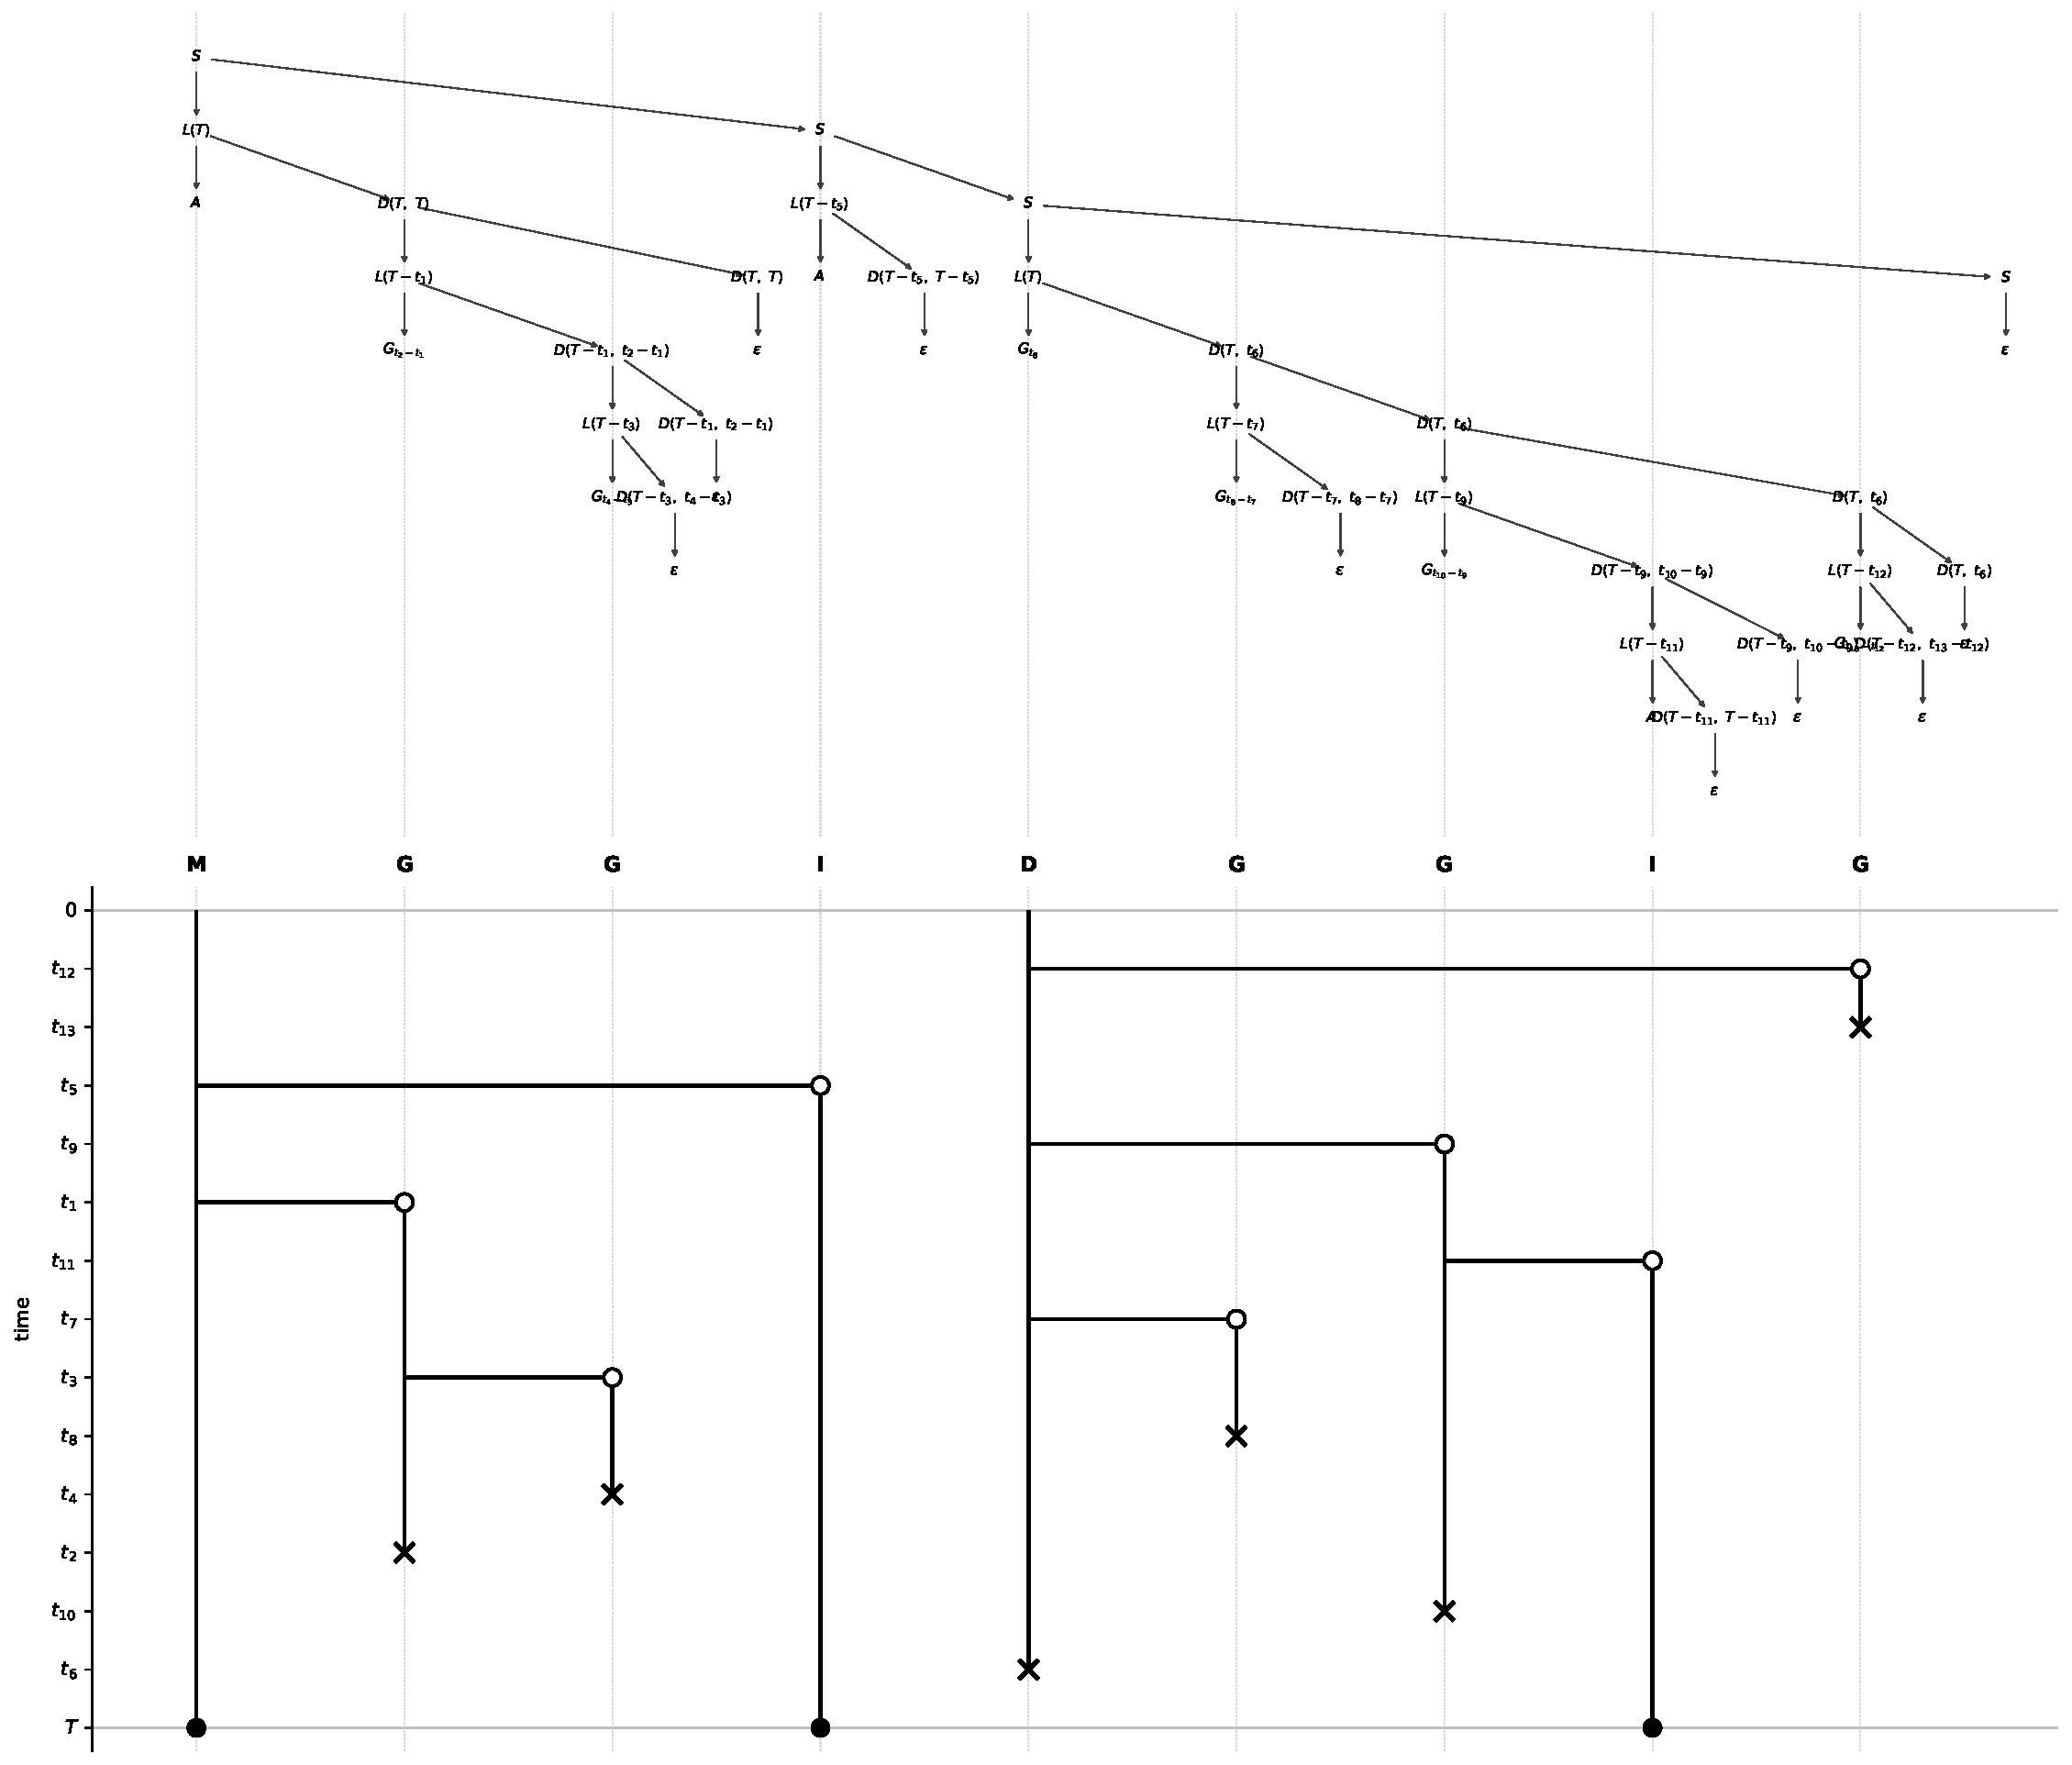
\includegraphics[width=0.75\linewidth]{tkf_trajectory_gravestone.pdf}
\caption{\textbf{TKF91 indel trajectory as a Galton--Watson branching
process and its gravestone-augmented SCFG parse tree.}
\textit{Top:} the gravestone-augmented SCFG parse tree of
\eqref{eq:gw-scfg} with $(t,T)$ annotations; each leaf terminal
($A$ for an alive residue, $G_\ell$ for a ghost) sits directly
above its trajectory column. \textit{Bottom:} one realization of the continuous-time TKF91 process on
a branch of length $T$; columns are residue lineages, $\circ$ = birth,
$\bullet$ = survival to the endpoint, $\times$ = death; ghost
$\mathrm{G}$ lineages are transient, living and dying within $(0,T)$ and
so leaving no trace at the endpoints.}
\label{fig:tkf-trajectory}
\end{figure}

The Inside matrix for this grammar can be computed using a generating function approach.
The posterior over trajectories, conditioned on a given alignment, can then be sampled
by stochastic traceback of a parse tree, as described in Appendix~\ref{appendix:sampling_scfg}.

% =============================================================
\section{Results: \Pfam\ fits and BAliBASE accuracies}
\label{sec:results}
% =============================================================

We fit TKF92 (\MixFrag, $\mathcal F{=}1$) and \MixFrag\ $\mathcal F{=}2$ by
exact summarized-count EM (\Cref{sec:cherryem}), and \MixDom-d3f1 by \svibw\
(\Cref{sec:svibw}), on a common \Pfam\ dataset.
We present two simpler mixtures as comparison points: CherryML-$C{=}20$, a 20-component mixture of substitution models (with one TKF92 indel model); and TKF92-$K{=}20$, a 20-component mixture of standard TKF92 indel models.
Both are also fit with exact summarized-count EM.
For all models, we use LG08 as our substitution model, with $(Q,\eqm)$ fixed to values from~\citet{LG08}.
The training split contains 20{,}897 families and
1{,}134{,}482 cherries.
The held-out validation split contains 2{,}293 families and 116{,}640 pairs.
\Cref{tab:pfam} reports the validation likelihood scored by two methods:
\emph{path-conditioned} (sum along the alignment) and
\emph{order-summed} (2D Forward; matches fixed but indel orderings summed).

\begin{table}[t]
\caption{Held-out per-pair log-likelihood
(nats) on the \Pfam\ validation split (116{,}640 pairs / 2{,}293
families); models trained as per \Cref{sec:results}. 
 Path-conditioned scoring fixes the order of insertions and deletions within each gap. Order-summed scoring sums over all possible orderings. }
\label{tab:pfam}
\centering
%\footnotesize
\setlength{\tabcolsep}{5pt}
\begin{tabular}{@{}lcc@{}}
\toprule
Model & path-cond. & \textbf{order-summed} \\
\midrule
TKF92 ($\mathcal F{=}1$) & $-726.30$ & $-721.97$ \\
\MixFrag\ $\mathcal F{=}2$ & $-726.44$ & $-720.09$ \\
\MixDom-d3f1 & $\mathbf{-718.57}$ & $\mathbf{-713.02}$ \\
\bottomrule
\end{tabular}
\end{table}

%Both models converge to
%$\kappa\approx0.98$, essentially the same birth--death process, so the
%mixture acts on fragment geometry not the indel rate:
\MixFrag\ splits
TKF92's single fragment-extension probability $r{=}0.677$ into a short mode ($r{\approx}0.375$,
weight $0.63$) and a long mode ($r{\approx}0.833$, weight $0.37$). 
The order-summed score exceeds the path-conditioned one for every model, by 4.3 nats/pair for TKF92 and 6.4 for \MixFrag.
\MixFrag\ is close to TKF92 when fitting \Pfam\ alignments as given (i.e. path-conditioned), but outperforms TKF92 when fitting unaligned \Pfam\ sequences (i.e. order-summed).

\subsection{Downstream alignment on BAliBASE}

To check that these trainers yield usable alignment models, we fed their
posteriors to a sequence annealing aligner~\cite{BradleyEtAl2009} and scored the merged
multiple alignments against BAliBASE (\Cref{tab:balibase}). \MixFrag\ ($\mathcal F{=}2$)
already improves on TKF92 across all three metrics. \MixDom-d3f1 improves further,
outperforming MAFFT on
all accuracy metrics.
 %($F_1$ $0.387$ vs.\ $0.377$, SP $0.812$ vs.\ $0.776$, TC $0.677$ vs.\ $0.622$);
A $K{=}20$ mixture of TKF92 models and the
20-class site mixture (CherryML-$C{=}20$) also edge out standard TKF92. 
All models were trained with counts-based exact EM except for \MixDom, which used \svibw.

\begin{table}[t]
\caption{Full-length BAliBASE
\texttt{bali3pdbm} alignment accuracy (120 families): soft posteriors
merged into a multiple alignment by an FSA aligner, scored by column
$F_1$, sum-of-pairs (SP) and total-column (TC). Top block: this paper's
trained models; bottom block: MAFFT and MUSCLE~\cite{Katoh2013,Edgar2004}.}
\label{tab:balibase}
\centering
%\footnotesize
\setlength{\tabcolsep}{5pt}
\begin{tabular}{@{}lccc@{}}
\toprule
Method & $F_1$ & SP & TC \\
\midrule
TKF92            & 0.377 & 0.776 & 0.622 \\
\MixFrag\ $\mathcal F{=}2$ & 0.384 & 0.790 & 0.640 \\
\MixDom-d3f1     & \textbf{0.387} & \textbf{0.812} & \textbf{0.677} \\
TKF92-$K{=}20$   & 0.378 & 0.784 & 0.633 \\
CherryML-$C{=}20$ & 0.384 & 0.791 & 0.645 \\
\midrule
MAFFT (FFT-NS-2) & 0.365 & 0.797 & 0.653 \\
MUSCLE (default) & 0.373 & 0.841 & 0.715 \\
\bottomrule
\end{tabular}
\end{table}

% =============================================================
\section{Discussion}
\label{sec:discussion}
% =============================================================

TKF-family models are exponential families with additive sufficient
statistics, so their M-steps are closed-form.
We have shown how to recover the relevant E-statistics via the score function identity;
the technique amounts, straightforwardly, to automatic differentiation of the Forward likelihood.
This directly supports approaches that augment the TKF models, whether by introducing latent structure
or by making the indel rates functions of the data~\cite{LargeHolmes2026}.

% Do NOT include this section in the anonymized submission, only in the final paper. You can use the \texttt{ack} environment provided in the style file to automatically hide this section in the anonymized submission.
% \begin{ack}
% We thank Jeff Thorne, Jotun Hein, Marc Suchard, Nicola De Maio, Elena Rivas, Sean Eddy, and David MacKay.
% Mathematics and code were generated by Anthropic's Claude under human supervision. Funded by NIH grants HG004483, GM080203, and HG013117.
% \end{ack}

%% References follow the acknowledgments and do not count towards the page
%% limit.  natbib+plainnat sets the unnumbered "References" heading itself.
%% The .bib file lives in this directory.
\newpage
\bibliographystyle{plainnat}
\bibliography{refs}


%%%%%%%%%%%%%%%%%%%%%%%%%%%%%%%%%%%%%%%%%%%%%%%%%%%%%%%%%%%%

\newpage
\appendix

%%% There were a lot of issues raised here, so removing for now
%\section{Transition probability for general BDI}
%\label{appendix:general_bdi}
%\newcommand\expect{\mathbb{E}}
%\newcommand\xpath{\mathbb{X}}
%\newcommand\insrate{\lambda}
%\newcommand\delrate{\mu}
%\newcommand\immrate{\nu}
%\newcommand{\ind}{\mathrm{ind}}
%\newcommand{\imm}{\mathrm{imm}}

%For the general linear BDI process with per-capita birth rate $\insrate$,
%per-capita death rate $\delrate$, and constant immigration rate $\immrate$
%(where $\immrate$ is a free parameter, not necessarily $0$ or $\insrate$),
%the transition probability $P_{ij}(T) = P(X(T) = j \mid X(0) = i)$ is known in closed form
%\cite{Kendall1948}.

%Using the $\alpha$ and $\beta$ from \eqref{eq:abg},
%define $\rho = \immrate / \insrate$ (the immigration-to-birth ratio).
%The transition probability factorizes as:
%\begin{equation}\label{eq:pij-general}
%P_{ij}(T) = \underbrace{P_{ij}^{(0)}(T)}_{\text{no-immigration}} \cdot
%\underbrace{R_{ij}(T)}_{\text{immigration factor}}
%\end{equation}
%The no-immigration factor is
%\begin{equation}\label{eq:pij-noimm}
%P_{ij}^{(0)}(T) = \sum_{k=0}^{\min(i,j)} \binom{i}{k} \binom{j-1}{k-1}
 % \alpha^k (1-\alpha)^{i-k} (1-\gamma)^{i-k}
 % \gamma^{j-k} (1-\beta)^{k+1} \beta^{j-k-1} \cdot \delta_{j>0}
%\end{equation}
%(with the $k=0$ term understood as $(1-\alpha)^i (1-\gamma)^i$ when $j=0$,
%and the convention $\binom{-1}{-1} = 1$).

%For the immigration factor,
%when $\immrate \neq \insrate$ (i.e.\ $\rho \neq 1$):
%\begin{equation}\label{eq:imm-factor}
%R_{ij}(T) = (1-\beta)^{\rho} \cdot
%{}_2F_1\!\left(-j, \rho;\, 1;\, \frac{\beta}{1-\beta} \cdot \frac{1}{\beta/(1-\beta)}\right)
%\end{equation} % AL: Don't these cancel, so it's just 1?
%More explicitly, the full $P_{ij}(T)$ with immigration can be written
%using the negative binomial form \cite{Kendall1948}:
%\begin{equation}\label{eq:pij-full}
%P_{ij}(T) = \sum_{k=0}^{\min(i,j)}
% \binom{i}{k}\binom{j-1}{k-1}
%  \alpha^k (1-\alpha-\gamma+\alpha\gamma)^{i-k}
%  \gamma^{j-k}(1-\beta)^{k+1}\beta^{j-k-1}
%  \cdot (1-\beta)^{\rho}
%  \sum_{m=0}^{j-k} \binom{\rho+m-1}{m}\beta^m
%\end{equation}
%where the inner sum is a truncated negative binomial in $\beta$ with parameter $\rho$.
%When $\rho = 1$ (i.e.\ $\immrate = \insrate$),
%the immigration factor simplifies to a factor of $(1-\beta)$, recovering the TKF91 transition probabilities.
%When $\rho = 0$ (no immigration), $R = 1$ and we recover $P_{ij}^{(0)}$.

%\subsection{\texorpdfstring{Score derivatives for $\immrate$}{Score derivatives for nu}}

%The score with respect to $\immrate$ is
%\[
%\frac{\partial}{\partial\immrate}\log P_{ij}
%= \frac{1}{P_{ij}} \frac{\partial P_{ij}}{\partial\immrate}
%\]
%Since $\immrate$ enters through $\rho = \immrate/\insrate$ and the factor $(1-\beta)^\rho$
%times the negative binomial sum, we have
%\begin{equation}
%\frac{\partial}{\partial\immrate}\log P_{ij}
%= \frac{1}{\insrate}\left(
%\log(1-\beta) + \psi(\rho) \cdot [\text{correction from the sum}]
%\right)
%\end{equation}
%where $\psi$ is the digamma function (arising from $\partial/\partial\rho\;\binom{\rho+m-1}{m}$).
%The full expression is:
%\begin{equation}\label{eq:dlogP-dnu}
%\frac{\partial}{\partial\immrate}\log P_{ij} = \frac{1}{\insrate}
%  \frac{\sum_k (\cdots) \sum_m \binom{\rho+m-1}{m}\beta^m
%  \left[\log(1-\beta) + \sum_{\ell=0}^{m-1}\frac{1}{\rho+\ell}\right]}
%  {\sum_k (\cdots) \sum_m \binom{\rho+m-1}{m}\beta^m}
%\end{equation}
%where $(\cdots)$ abbreviates the terms from the outer sum in~(\ref{eq:pij-full}).

\section{The substitution model M-step}

\newcommand\expect{\mathbb{E}}
\newcommand\xpath{\mathbb{X}}
\newcommand\insrate{\lambda}
\newcommand\delrate{\mu}
\newcommand\immrate{\nu}
\newcommand{\ind}{\mathrm{ind}}
\newcommand{\imm}{\mathrm{imm}}

\label{appendix:subst-mstep}
The closed-form M-step is a property of the indel process; the substitution side is more nuanced.
Some substitution models do have closed-form MLEs
from the expected transition counts and dwell
times~\cite{HolmesRubin2002,HobolthJensen2005,HobolthJensen2011};
these include unconstrained (irreversible) models and reversible models whose parameters decouple from the
reversibility constraint (F81, JC69, K80, HKY). Write
$U_{ij}$ for the expected number of $i{\to}j$ substitutions and $W_i$ for
the expected dwell time in state $i$ (the endpoint-conditioned CTMC
expectations, delivered by the same score identity),
and restrict for simplicity to the conditional case $P(y \mid x)$.
The unconstrained-generator MLE is $\hat Q_{ij}=U_{ij}/W_i$ and the
reversible (detailed-balance) exchangeability MLE is
\begin{equation*}
\hat\theta_{ij}=\frac{U_{ij}+U_{ji}}{W_i\,\pi_j+W_j\,\pi_i},
\end{equation*}
pooled over symmetry classes for JC69/K80/F81/HKY. The general reversible
GTR instead requires iteration, since $Q_{ij}=\theta_{ij}\pi_j$ couples the
exchangeabilities to the equilibrium: a suitable approach is to alternate the
$\theta$-update with recomputing $\pi$. Those expectations also depend on
when indels fell on a branch, requiring genealogical corrections whose
exact treatment via the gravestone construction of \Cref{sec:gravestone}
we leave open; we assume the perturbation is negligible. 

\section{\svibw\ implementation analyses}
\label{appendix:svibw_appendix}

\subsection{How much data? Effective sample size is counted in pairs}
The estimator's precision is set by the Fisher information per pair,
and for indel rates the accounting differs from substitution.
Write $n$ for the total number of sequence pairs processed: the
minibatch size times the number $K$ of iterations. By the delta method,
for $n$ independent pairs,
\begin{equation}
\label{eq:relvar}
\frac{\mathrm{Var}[\hat\ins]}{\ins^2}\approx\frac{v_\ins}{n},\qquad
v_\ins=\frac{\sigma_B^2}{\E[B]^2}+\frac{\sigma_S^2}{(\E[S]+t)^2}
        -\frac{2\,\mathrm{Cov}[B,S]}{\E[B](\E[S]+t)} .
\end{equation}
One might hope to buy precision from \emph{longer} alignments rather than
from \emph{more} pairs. Conditioned on the ancestor length $i$, the links
evolve as independent sub-lineages, so the Fisher information for $\ins$
does grow linearly in $i$: at fixed $i$ a longer pair is genuinely more
informative, $v_\ins(i)=\Theta(1/i)$. This cannot be exploited, however,
because at stationarity the length is not a free variable; the model pins
it at mean $\kappa/(1{-}\kappa)$. Each pair therefore carries a fixed
expected information, the length distribution drops out of $v_\ins$ at
first order (the ratio $\E[B\mid i]/(\E[S\mid i]{+}t)=\ins$ is exactly
constant in $i$), and the effective sample size is simply the number of
pairs. A
rule of thumb is $v_\theta\approx 5$ for typical protein regimes
($\kappa\approx0.9$, $t\approx1$), giving the sample budget
$n\gtrsim v_\theta/\varepsilon^2$ for target relative error
$\varepsilon$ (e.g.\ $n\approx400\,v_\theta$ for $\varepsilon{=}0.05$).

\subsection{Averaging and step size: rare events dominate the convergence tail}
\label{sub:averaging}

Treating \svibw\ as stochastic approximation~\cite{cappemoulines2009},
three regimes differ only in how the M-step output is smoothed. With a
direct M-step (no smoothing), the parameter's asymptotic variance stays
at the single-minibatch level and does \emph{not} shrink with the number
of iterations; an EMA of rate $\eta$ scales it by $\tfrac{\eta}{2-\eta}$;
and Polyak--Ruppert averaging of the iterates attains
$\mathrm{Var}[\bar\theta]\approx\Sigma/n$, the optimal $1/\sqrt{n}$ error
in the total pair count $n$. We therefore run a decreasing
step schedule ($\eta_k\propto 1/(k{+}2)$) with a Polyak average of the
tail. Parameter groups fed by rare events, such as fragtypes present in
a fraction $\epsilon$ of minibatches, have effective sample size
$\epsilon$ times smaller and dominate the convergence tail (the $w_f$
updates converge last), as the Dirichlet--multinomial Hessian
$\mathrm{diag}(1/\alpha_i)$ predicts.


% ==============================================================
% Self-contained appendix: Exploded MixDom Pair HMM
% Assembled from tkf-mixdom/tkf/exploded-mixdom.tex (lines 9-247)
% plus the macro definitions it uses, from tkf/preamble-shared.tex.
%
% Package requirements: amsmath, array (for >{\raggedright\arraybackslash}p{})
%                       enumitem (for \begin{itemize}[nosep])
% ==============================================================

% ---- macros (from preamble-shared.tex; move to your preamble) ----
\newcommand\anctok{a}
\newcommand\class{c}
\newcommand\classdist{u}                % per-(domain,fragtype) class distribution
\newcommand{\deldel}{\mathtt{DD}}
\newcommand{\deldom}{\mathtt{DelDom}}
\newcommand{\deldomend}{\mathtt{DelDomEnd}}
\newcommand{\deldomtype}[1]{\mathtt{DelDomType}[#1]}
\newcommand\delstate{{\tt D}}
\newcommand\destdom{d^\prime}
\newcommand\destok{b}
\newcommand{\dkfrag}[1]{\mathtt{DFrag}[#1]}
\newcommand{\dkfragemit}[1]{\mathtt{DEmit}[#1]}
\newcommand{\dkfragend}[1]{\mathtt{DFragEnd}[#1]}
\newcommand{\dkfragtype}[1]{\mathtt{DFragType}[#1]}
\newcommand\domenter{p_\mathrm{in}}
\newcommand\domexit{p_\mathrm{out}}
\newcommand\evoltime{t}              % section 6 uses t
\newcommand\fin{{\tt E}}
\newcommand{\ikfrag}[1]{\mathtt{IFrag}[#1]}
\newcommand{\ikfragemit}[1]{\mathtt{IEmit}[#1]}
\newcommand{\ikfragend}[1]{\mathtt{IFragEnd}[#1]}
\newcommand{\ikfragtype}[1]{\mathtt{IFragType}[#1]}
\newcommand{\insdom}{\mathtt{InsDom}}
\newcommand{\insdomend}{\mathtt{InsDomEnd}}
\newcommand{\insdomtype}[1]{\mathtt{InsDomType}[#1]}
\newcommand{\insins}{\mathtt{II}}
\newcommand\insstate{{\tt I}}
\newcommand\mat{{\tt M}}
\newcommand{\matdel}{\mathtt{MD}}
\newcommand{\matdom}{\mathtt{MatDom}}
\newcommand{\matdomend}{\mathtt{MatDomEnd}}
\newcommand{\matdomtype}[1]{\mathtt{MatDomType}[#1]}
\newcommand{\matins}{\mathtt{MI}}
\newcommand{\matmat}{\mathtt{MM}}
\newcommand{\mkdfrag}[1]{\mathtt{DelFrag}[#1]}
\newcommand{\mkdfragemit}[1]{\mathtt{DelEmit}[#1]}
\newcommand{\mkdfragend}[1]{\mathtt{DelFragEnd}[#1]}
\newcommand{\mkdfragtype}[1]{\mathtt{DelFragType}[#1]}
\newcommand{\mkfrag}[1]{\mathtt{MatFrag}[#1]}
\newcommand{\mkfragemit}[1]{\mathtt{MatEmit}[#1]}
\newcommand{\mkfragend}[1]{\mathtt{MatFragEnd}[#1]}
\newcommand{\mkfragtype}[1]{\mathtt{MatFragType}[#1]}
\newcommand{\mkifrag}[1]{\mathtt{InsFrag}[#1]}
\newcommand{\mkifragemit}[1]{\mathtt{InsEmit}[#1]}
\newcommand{\mkifragend}[1]{\mathtt{InsFragEnd}[#1]}
\newcommand{\mkifragtype}[1]{\mathtt{InsFragType}[#1]}
\newcommand\nclasses{C}
\newcommand\ndom{N}                  % section 6: N domain types
\newcommand\nonemptytrans{\Aeff}
\newcommand\notext{\bar r}           % rho is the DOMAIN weight in section 6
\newcommand\revsub{R}
\newcommand\samedom{\delta(\srcdom=\destdom)}
\newcommand\srcdom{d}                % section 6 domain index
\newcommand\sta{{\tt S}}
\newcommand\tkftrans{\tau}
\newcommand\ustate{{\tt U}}
\newcommand\vstate{{\tt V}}
\newcommand\xstate{{\tt X}}
\newcommand\ystate{{\tt Y}}

% ---- content ----
\section{Exploded MixDom pair HMM}
\label{appendix:exploded-mixdom}

\subsection{State space}

The exploded MixDom Pair HMM makes every structural decision explicit
as a separate state transition. Let $\ndom$ denote the number of domain
types; there is a single fragment type per domain, so parameters are indexed
by domain type $d$ alone.

The states are shown in Table~\ref{tab:exploded-state-space}.

\begin{table}[t]
\centering
\caption{Exploded MixDom Pair HMM state space.}
\label{tab:exploded-state-space}
\begin{tabular}{>{\raggedright\arraybackslash}p{0.35\linewidth} >{\raggedright\arraybackslash}p{0.45\linewidth} >{\raggedleft\arraybackslash}p{0.10\linewidth}}
\hline
\textbf{Category} & \textbf{States} & \textbf{Count} \\
\hline
\textbf{Start/End}
& $\sta$, $\fin$ & $2$ \\

\makecell[l]{\textbf{Domain-level}\\(top-level TKF91 states)}
& $\matdom$, $\insdom$, $\deldom$, $\matdomend$, $\insdomend$, $\deldomend$ & $6$ \\

\makecell[l]{\textbf{Domain type selection}\\(one per domain type $d$)}
& $\matdomtype{d}$, $\insdomtype{d}$, $\deldomtype{d}$ & $3\ndom$ \\

\makecell[l]{\textbf{Fragment-level}\\(inner TKF states\\within $\matdomtype{d}$)}
& $\mkfrag{d}$, $\mkifrag{d}$, $\mkdfrag{d}$ & $3\ndom$ \\

\makecell[l]{\textbf{Fragment-level}\\(single looping state within\\$\insdomtype{d}$, $\deldomtype{d}$)}
& $\ikfrag{d}$, $\dkfrag{d}$ & $2\ndom$ \\

\makecell[l]{\textbf{Fragment type selection}\\(weight-one, single fragment type)}
& $\mkfragtype{d}$, $\mkifragtype{d}$, $\mkdfragtype{d}$,
  $\ikfragtype{d}$, $\dkfragtype{d}$ & $5\ndom$ \\

\makecell[l]{\textbf{Emit states}\\(the only emitting states)}
& $\mkfragemit{d}$, $\mkifragemit{d}$, $\mkdfragemit{d}$,
  $\ikfragemit{d}$, $\dkfragemit{d}$ & $5\ndom$ \\

\makecell[l]{\textbf{Fragment end}\\(fragment termination)}
& $\mkfragend{d}$, $\mkifragend{d}$, $\mkdfragend{d}$,
  $\ikfragend{d}$, $\dkfragend{d}$ & $5\ndom$ \\
\hline
\textbf{Total} & \multicolumn{2}{r}{$8 + 23\ndom$} \\
\hline
\end{tabular}
\end{table}

The emitting states correspond to the compound states of the collapsed model:
$\mkfragemit{d} = \matmat_d$, $\mkifragemit{d} = \matins_d$,
$\mkdfragemit{d} = \matdel_d$, $\ikfragemit{d} = \insins_d$,
$\dkfragemit{d} = \deldel_d$.

\subsection{Transition weights}

All transitions are between non-emitting states, or from non-emitting to
emitting, or from emitting to non-emitting (Mealy machine: emissions occur
on the transitions into emit states).

We use BDI parameters for two TKF91 processes:
\begin{itemize}[nosep]
\item Top-level (domain sequence): $\alpha_*, \beta_*, \gamma_*, \kappa_*$
  from $(\insrate_*, \delrate_*, \evoltime)$
\item Per-domain $d$ (fragment sequence): $\alpha_d, \beta_d, \gamma_d, \kappa_d$
  from $(\insrate_d, \delrate_d, \evoltime)$
\end{itemize}

\subsubsection{Top-level transitions}

These implement the TKF91 Pair HMM structure with $\matdom/\insdom/\deldom/\fin$ (for incoming connections) and $\sta/\matdomend/\insdomend/\deldomend$ (for outgoing connections)
playing the roles of $\sta/\mat/\insstate/\delstate/\fin$:
\begin{align}
\sta &\to \matdom: \quad \tkftrans_{\sta\mat}(\insrate_*,\delrate_*,\evoltime) \\
\sta &\to \insdom: \quad \tkftrans_{\sta\insstate}(\insrate_*,\delrate_*,\evoltime) \\
\sta &\to \deldom: \quad \tkftrans_{\sta\delstate}(\insrate_*,\delrate_*,\evoltime) \\
\sta &\to \fin: \quad \tkftrans_{\sta\fin}(\insrate_*,\delrate_*,\evoltime) \\
\matdomend &\to \matdom: \quad \tkftrans_{\mat\mat}(\insrate_*,\delrate_*,\evoltime) \\
\matdomend &\to \insdom: \quad \tkftrans_{\mat\insstate}(\insrate_*,\delrate_*,\evoltime) \\
\matdomend &\to \deldom: \quad \tkftrans_{\mat\delstate}(\insrate_*,\delrate_*,\evoltime) \\
\matdomend &\to \fin: \quad \tkftrans_{\mat\fin}(\insrate_*,\delrate_*,\evoltime) \\
\insdomend &\to \matdom: \quad \tkftrans_{\insstate\mat}(\insrate_*,\delrate_*,\evoltime) \\
\insdomend &\to \insdom: \quad \tkftrans_{\insstate\insstate}(\insrate_*,\delrate_*,\evoltime) \\
\insdomend &\to \deldom: \quad \tkftrans_{\insstate\delstate}(\insrate_*,\delrate_*,\evoltime) \\
\insdomend &\to \fin: \quad \tkftrans_{\insstate\fin}(\insrate_*,\delrate_*,\evoltime) \\
\deldomend &\to \matdom: \quad \tkftrans_{\delstate\mat}(\insrate_*,\delrate_*,\evoltime) \\
\deldomend &\to \insdom: \quad \tkftrans_{\delstate\insstate}(\insrate_*,\delrate_*,\evoltime) \\
\deldomend &\to \deldom: \quad \tkftrans_{\delstate\delstate}(\insrate_*,\delrate_*,\evoltime) \\
\deldomend &\to \fin: \quad \tkftrans_{\delstate\fin}(\insrate_*,\delrate_*,\evoltime)
\end{align}

\subsubsection{Domain type selection}

\begin{align}
\matdom &\to \matdomtype{d}: \quad \rho_d \quad\text{(domain weight)} \\
\insdom &\to \insdomtype{d}: \quad \rho_d \\
\deldom &\to \deldomtype{d}: \quad \rho_d
\end{align}

\subsubsection{Domain-to-fragment entry (M-type domains)}

Within $\matdomtype{d}$, the fragment-level TKF91 begins.
Again, this follows the TKF91 Pair HMM structure, now with $\mkfrag{d}/\mkifrag{d}/\mkdfrag{d}/\matdomend$ (for incoming connections) and $\matdomtype{d}/\mkfragend{d}/\mkifragend{d}/\mkdfragend{d}$ states (for outgoing connections)
playing the roles of $\sta/\mat/\insstate/\delstate/\fin$:
\begin{align}
\matdomtype{d} &\to \mkfrag{d}: \quad \tkftrans_{\sta\mat}(\insrate_d,\delrate_d,\evoltime) \\
\matdomtype{d} &\to \mkifrag{d}: \quad \tkftrans_{\sta\insstate}(\insrate_d,\delrate_d,\evoltime) \\
\matdomtype{d} &\to \mkdfrag{d}: \quad \tkftrans_{\sta\delstate}(\insrate_d,\delrate_d,\evoltime) \\
\matdomtype{d} &\to \matdomend: \quad \tkftrans_{\sta\fin}(\insrate_d,\delrate_d,\evoltime) \\
\mkfragend{d} &\to \mkfrag{d}: \quad \tkftrans_{\mat\mat}(\insrate_d,\delrate_d,\evoltime) \\
\mkfragend{d} &\to \mkifrag{d}: \quad \tkftrans_{\mat\insstate}(\insrate_d,\delrate_d,\evoltime) \\
\mkfragend{d} &\to \mkdfrag{d}: \quad \tkftrans_{\mat\delstate}(\insrate_d,\delrate_d,\evoltime) \\
\mkfragend{d} &\to \matdomend: \quad \tkftrans_{\mat\fin}(\insrate_d,\delrate_d,\evoltime) \\
\mkifragend{d} &\to \mkfrag{d}: \quad \tkftrans_{\insstate\mat}(\insrate_d,\delrate_d,\evoltime) \\
\mkifragend{d} &\to \mkifrag{d}: \quad \tkftrans_{\insstate\insstate}(\insrate_d,\delrate_d,\evoltime) \\
\mkifragend{d} &\to \mkdfrag{d}: \quad \tkftrans_{\insstate\delstate}(\insrate_d,\delrate_d,\evoltime) \\
\mkifragend{d} &\to \matdomend: \quad \tkftrans_{\insstate\fin}(\insrate_d,\delrate_d,\evoltime) \\
\mkdfragend{d} &\to \mkfrag{d}: \quad \tkftrans_{\delstate\mat}(\insrate_d,\delrate_d,\evoltime) \\
\mkdfragend{d} &\to \mkifrag{d}: \quad \tkftrans_{\delstate\insstate}(\insrate_d,\delrate_d,\evoltime) \\
\mkdfragend{d} &\to \mkdfrag{d}: \quad \tkftrans_{\delstate\delstate}(\insrate_d,\delrate_d,\evoltime) \\
\mkdfragend{d} &\to \matdomend: \quad \tkftrans_{\delstate\fin}(\insrate_d,\delrate_d,\evoltime)
\end{align}

The $\matdomtype{d} \to \matdomend$ transition is the ``phantom''
null path: the domain is entered but the inner model immediately terminates
with no fragments emitted. This leads to null cycles that must be eliminated by Schur complement.

\subsubsection{Domain-to-fragment entry (I/D-type domains)}

$\insdomtype{d}$ and $\deldomtype{d}$ have a single looping fragment state:
\begin{align}
\insdomtype{d} &\to \ikfrag{d}: \quad \kappa_d \\
\insdomtype{d} &\to \insdomend: \quad 1 - \kappa_d \\
\deldomtype{d} &\to \dkfrag{d}: \quad \kappa_d \\
\deldomtype{d} &\to \deldomend: \quad 1 - \kappa_d
\end{align}

Again, the $\to \insdomend / \deldomend$ transitions are null (empty domain).

\subsubsection{Fragment type selection (trivial for one fragtype)}

With a single fragment type the fragtype weight is $w_{d1}=1$, so these
transitions are weight-one pass-throughs, retained only to keep the emission
transitions (below) distinct from the fragment-entry transitions:
\begin{align}
\mkfrag{d} &\to \mkfragtype{d}: \quad 1 \\
\mkifrag{d} &\to \mkifragtype{d}: \quad 1 \\
\mkdfrag{d} &\to \mkdfragtype{d}: \quad 1 \\
\ikfrag{d} &\to \ikfragtype{d}: \quad 1 \\
\dkfrag{d} &\to \dkfragtype{d}: \quad 1
\end{align}

\subsubsection{Fragment emission}

These are the only transitions with emissions (the exploded HMM is represented as a Mealy machine, so emissions occur on transitions; the collapsed HMM treats emissions as state-based).
The emission probability is summed over site classes $\class \in \{1,\ldots,\nclasses\}$,
weighted by the per-domain class distribution $\classdist_{d\class}$:
\begin{align}
\mkfragtype{d} &\xrightarrow{(\anctok,\destok)} \mkfragemit{d}: \quad \sum_{\class=1}^{\nclasses} \classdist_{d\class}\, \eqm^{(\class)}_\anctok \exp(\revsub^{(\class)} \evoltime)_{\anctok\destok}
  \quad\text{(align $(\anctok,\destok)$)} \\
\mkifragtype{d} &\xrightarrow{(\epsilon,\destok)} \mkifragemit{d}: \quad \sum_{\class=1}^{\nclasses} \classdist_{d\class}\, \eqm^{(\class)}_\destok
  \quad\text{(insert $\destok$)} \\
\mkdfragtype{d} &\xrightarrow{(\anctok,\epsilon)} \mkdfragemit{d}: \quad \sum_{\class=1}^{\nclasses} \classdist_{d\class}\, \eqm^{(\class)}_\anctok
  \quad\text{(delete $\anctok$)} \\
\ikfragtype{d} &\xrightarrow{(\epsilon,\destok)} \ikfragemit{d}: \quad \sum_{\class=1}^{\nclasses} \classdist_{d\class}\, \eqm^{(\class)}_\destok
  \quad\text{(insert $\destok$)} \\
\dkfragtype{d} &\xrightarrow{(\anctok,\epsilon)} \dkfragemit{d}: \quad \sum_{\class=1}^{\nclasses} \classdist_{d\class}\, \eqm^{(\class)}_\anctok
  \quad\text{(delete $\anctok$)}
\end{align}

\subsubsection{Fragment extension vs.\ fragment termination}
\label{sec:mixdom-frag-trans}

Within each fragment of domain $d$ the process either extends the current
fragment, with probability $\ext_d$, or terminates it, with probability
$1-\ext_d$. Different fragments are statistically independent. The
extension transition returns to the fragment's type-selection state, from
which the next position is emitted:
\begin{align}
\mkfragemit{d} &\to \mkfragtype{d}: \quad \ext_d \quad\text{(fragment extension)} \\
\mkfragemit{d} &\to \mkfragend{d}: \quad 1-\ext_d \quad\text{(fragment termination)} \\
\mkifragemit{d} &\to \mkifragtype{d}: \quad \ext_d  \\
\mkifragemit{d} &\to \mkifragend{d}: \quad 1-\ext_d  \\
\mkdfragemit{d} &\to \mkdfragtype{d}: \quad \ext_d  \\
\mkdfragemit{d} &\to \mkdfragend{d}: \quad 1-\ext_d  \\
\ikfragemit{d} &\to \ikfragtype{d}: \quad \ext_d  \\
\ikfragemit{d} &\to \ikfragend{d}: \quad 1-\ext_d  \\
\dkfragemit{d} &\to \dkfragtype{d}: \quad \ext_d  \\
\dkfragemit{d} &\to \dkfragend{d}: \quad 1-\ext_d
\end{align}
Fragment lengths within domain $d$ are therefore geometric with parameter
$\ext_d$, as in TKF92.

\subsection{Null state classification}

Every state except $\sta$, $\fin$, and the five emit states
$\mkfragemit{d}$, $\mkifragemit{d}$, $\mkdfragemit{d}$,
$\ikfragemit{d}$, $\dkfragemit{d}$ is a \textbf{null state}
(non-emitting). The collapsed model retains only $\sta$, $\fin$, and
the $5\ndom$ emit states.

\subsection{Null elimination}

The null states are eliminated by the standard HMM null closure:
\[
\bm{T}^{\rm nest} = \bm{T}^{\rm exp}_{\bar\varnothing\bar\varnothing}
+ \bm{T}^{\rm exp}_{\bar\varnothing\varnothing}\,\Zsum\,\bm{T}^{\rm exp}_{\varnothing\bar\varnothing},\qquad \Zsum = (\bm{I}-\Tnull)^{-1}
\]
Since there are no direct emit$\to$emit transitions in the exploded model
(every path between emit states passes through at least one null state),
$\bm{T}^{\rm exp}_{\bar\varnothing\bar\varnothing} = 0$ and:
\[
\bm{T}^{\rm nest} = \bm{T}^{\rm exp}_{\bar\varnothing\varnothing}\,\Zsum\,\bm{T}^{\rm exp}_{\varnothing\bar\varnothing}
\]

This gives the collapsed $\bm{T}^{\rm nest}$ matrix with states
$\{\sta, \fin, \matmat_d, \matins_d, \matdel_d, \insins_d, \deldel_d\}$,
matching the collapsed MixDom Pair HMM $\bm{T}^{\rm nest}$ of the main text.

Each state in the ($5\ndom$+2)-state collapsed HMM corresponds to an uneliminated state in the ($8+23\ndom$)-state exploded HMM: either $\sta$ ($\sta\sta$), $\fin$ ($\fin\fin$), or one of the emit states
$\mkfragemit{\srcdom}$ ($\matmat_{\srcdom}$), $\mkifragemit{\srcdom}$ ($\mat\insstate_{\srcdom}$), $\mkdfragemit{\srcdom}$ ($\mat\delstate_{\srcdom}$),
  $\ikfragemit{\srcdom}$ ($\insstate\insstate_{\srcdom}$), $\dkfragemit{\srcdom}$ ($\delstate\delstate_{\srcdom}$).
The transition weight from $\ustate\xstate_{\srcdom}$ to $\vstate\ystate_{\destdom}$ in the collapsed Pair HMM
has the form $\domexit(\ustate,\xstate,\srcdom) \times \nonemptytrans_{\ustate\vstate}(\ustate,\vstate) \times \domenter(\vstate,\ystate,\destdom) + \delta_{\ustate\vstate} \samedom (p_\text{SameDom}(\ustate,\xstate,\srcdom) + \delta_{\xstate\ystate} p_\text{SameFrag}(\srcdom))$
corresponding to the following path segments
\begin{itemize}
  \item $\domexit(\ustate,\xstate,\srcdom)$ represents transitions from the emit state to the end state of the domain, e.g. $\tkftrans_{\mat\fin}(\mat,\insstate,\srcdom)$ represents $\mkifragemit{\srcdom} \to \mkifragend{\srcdom} \to \matdomend$;
  \item $\nonemptytrans_{\ustate\vstate}(\ustate,\vstate)$ represents the sum over all paths from the domain end state (or $\sta$), through zero or more empty domains, to the next (nonempty) domain start (or $\fin$), e.g. $\nonemptytrans_{\mat\delstate}(\mat,\delstate)$ represents paths like $\matdomend \to (\ldots \insdom \to \insdomtype{d''} \to \insdomend \ldots )^\ast \to \deldom$. This is where null cycle elimination happens;
  \item $\domenter(\vstate,\ystate,\destdom)$ represents paths from the domain start state to an emit state inside the domain, e.g. $\tkftrans_{\sta\mat}(\mat,\insstate,\destdom)$ represents $\matdom \to \matdomtype{\destdom} \to \mkifrag{\destdom} \to \mkifragtype{\destdom}$;
  \item $p_\text{SameDom}(\xstate,\ystate,\srcdom)$ represents paths from the emit state to another emit state of similar profile but (potentially) different fragment type within the same domain, e.g. $p_\text{SameDom}(\mat,\insstate,\srcdom)$ represents $\mkifragemit{\srcdom} \to \matdomend \to \matdom \to \matdomtype{\srcdom} \to \mkifrag{\srcdom} \to \mkifragtype{\srcdom}$;
  \item $p_\text{SameFrag}(\srcdom) = \ext_{\srcdom}$ represents intra-fragment Markov transitions between fragment-types (extending the current fragment by one position). In this work, we restrict all fragment extensions to be between the same fragment type.
\end{itemize}

\section{Gravestone-augmented pair SCFG: sampling latent histories conditioned on observed alignments}
\label{appendix:sampling_scfg}
 
\subsection{Closing the sum: a bivariate generating function}
% changed variable name for "lifetime": tau -> ell
Sampling from this grammar requires the Inside weights, and these close
in a bivariate generating function of the alive and ghost counts.
Let $N_a(t)$, $N_g(t)$ be the numbers of alive and ghost lineages
after time $t$, and $f_t(z,w)=\E[z^{N_a(t)}w^{N_g(t)}]$ their joint PGF.
The Volterra fixed point
\begin{equation}
\label{eq:volterra}
f_t(z,w) = z\,e^{-\del t}\,\exp\!\Bigl(\ins\!\!\int_0^{t}\!\! (f_s - 1)\, ds\Bigr)
  + w\!\!\int_0^{t}\!\!\del e^{-\del\ell}\,\exp\!\Bigl(\ins\!\!\int_{t-\ell}^{t}\!\! (f_s - 1)\, ds\Bigr)\,d\ell
\end{equation}
is the Inside recursion of \eqref{eq:gw-scfg} in the $(z,w)$ domain: the
first term is the $A$ production (a surviving founder, contributing $z$),
the second the $G_\ell$ production (a ghost, contributing $w$)
integrated over its death time. It is equivalent to the forward equation
\begin{equation}
\label{eq:riccati}
\partial_t f_t = [\ins z^2 - (\ins{+}\del) z + \del w]\,\partial_z f_t,
\qquad f_0 = z,
\end{equation}
whose characteristic $\dot z=-[\ins z^2 - (\ins{+}\del)z + \del w]$
closes algebraically. Defining
$\Delta(w)=\sqrt{(\ins{-}\del)^2 + 4\ins\del(1-w)}$ and
$z_\pm(w)=((\ins{+}\del)\pm\Delta(w))/(2\ins)$, the characteristic
integrates to
\begin{equation}
\label{eq:riccati-flow}
\frac{z(t) - z_+}{z(t) - z_-}
= \frac{z(0) - z_+}{z(0) - z_-}\,e^{-\Delta(w)\, t},
\end{equation}
which inverts to give $f_t$, hence the pointwise joint $(N_a,N_g)$
distribution at any branch length; $w{=}1$ recovers the ordinary birth--death PGF for $N_a$
alone, while the marginal in $w$ is the ghost-count distribution
whose mean is the ghost mass named above.

\subsection{Drawing the history}
% changed variable name for "lifetime": tau -> ell
\Cref{eq:riccati-flow} gives closed-form per-branch transition kernels
in $(N_a,N_g)$ that compose across a tree: the count marginal at each
internal node is a closed-form pointwise distribution computable in
$O(1)$, so a Felsenstein-style upwards--downwards pass yields a
tree-level closed-form sampler, a \emph{phylogenetic} SCFG of the same
time-indexed form. To draw a history, one samples $(N_a,N_g)$ from the
closed-form midpoint marginal, then unrolls \eqref{eq:gw-scfg} top-down:
each sampled ghost $G_\ell$ is instantiated with its birth--death
time $\ell$ and, recursively, its own buried sublineage. The result is a
complete latent indel history whose alive residues match the observed
alignment and whose ghosts are imputed from their exact posterior.

\end{document}


